\documentclass[tikz,border=8pt]{standalone}
\usepackage{tikz}
\usetikzlibrary{decorations.pathreplacing}
\begin{document}
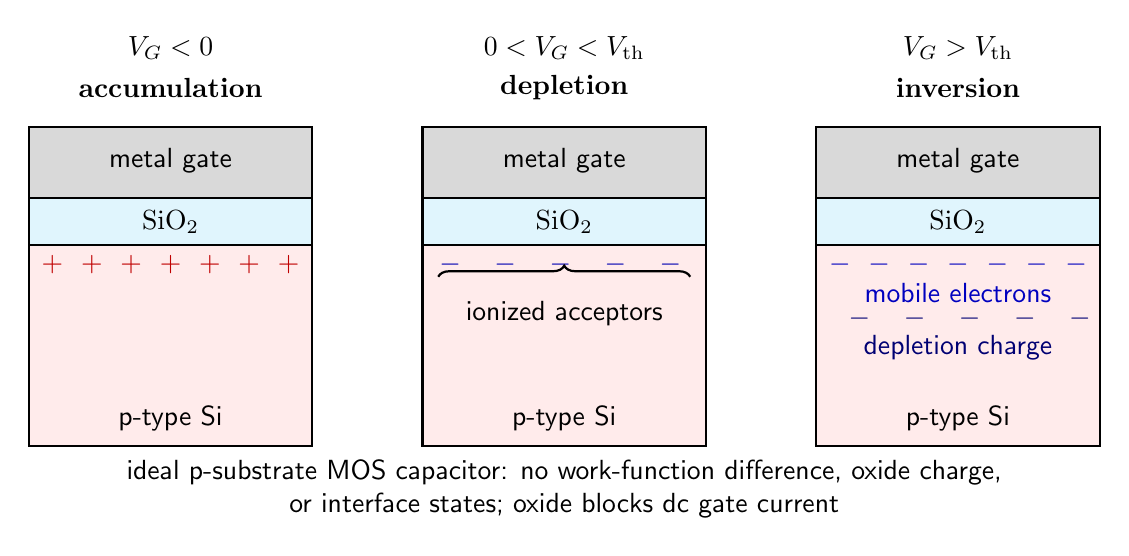
\begin{tikzpicture}[font=\sffamily]
\foreach \x/\ttl/\sgn in {0/accumulation/$V_G<0$,5/depletion/$0<V_G<V_{\rm th}$,10/inversion/$V_G>V_{\rm th}$}{
  \begin{scope}[shift={(\x,0)}]
    \fill[gray!30] (0,3.15) rectangle (3.6,4.05);
    \fill[cyan!12] (0,2.55) rectangle (3.6,3.15);
    \fill[red!8] (0,0) rectangle (3.6,2.55);
    \draw[thick] (0,0) rectangle (3.6,4.05);
    \draw[thick] (0,2.55)--(3.6,2.55) (0,3.15)--(3.6,3.15);
    \node at (1.8,3.62) {metal gate};
    \node at (1.8,2.84) {$\mathrm{SiO_2}$};
    \node at (1.8,0.35) {p-type Si};
    \node[font=\bfseries] at (1.8,4.55) {\ttl};
    \node at (1.8,5.05) {\sgn};
  \end{scope}
}
\foreach \x in {0.3,0.8,1.3,1.8,2.3,2.8,3.3}
  \node[red!75!black] at (\x,2.30) {$+$};
\foreach \x in {5.35,6.05,6.75,7.45,8.15}
  \node[blue!70!black] at (\x,2.30) {$-$};
\draw[decorate,decoration={brace,amplitude=4pt},thick] (5.2,2.15)--(8.4,2.15)
  node[midway,below=5pt] {ionized acceptors};
\foreach \x in {10.3,10.8,11.3,11.8,12.3,12.8,13.3}
  \node[blue!75!black] at (\x,2.30) {$-$};
\foreach \x in {10.55,11.25,11.95,12.65,13.35}
  \node[blue!45!black] at (\x,1.62) {$-$};
\node[blue!75!black] at (11.8,1.95) {mobile electrons};
\node[blue!45!black] at (11.8,1.25) {depletion charge};
\node[align=center] at (6.8,-0.55)
  {ideal p-substrate MOS capacitor: no work-function difference, oxide charge,\\or interface states; oxide blocks dc gate current};
\end{tikzpicture}
\end{document}
